\documentclass{book}

\usepackage{graphicx}
\usepackage{moreverb}
\usepackage{amsmath}
\usepackage{alltt}
\usepackage{rotating}
\usepackage{subfigure}
\usepackage{toc}
\usepackage{xspace}
\usepackage{makeidx}

\usepackage[T1]{fontenc}   % so _, <, and > print correctly in text.

\usepackage[strings]{underscore}    % to use "_" in text
\usepackage[dvips,colorlinks=true]{hyperref}   % Must be last package!

\newcommand{\sref}[1]{\S\ref{#1}}
\newcommand{\Sref}[1]{Sec.~\sref{#1}}

\newcommand{\vn}{\begingroup\catcode`\_=11 \catcode`\%=11 \dottcmd}
\newcommand\dottcmd[1]{{\usefont{T1}{lmss}{bx}{n} #1}\endgroup}

\newenvironment{example}
  {\vspace{-3.0ex} \begin{alltt}}
  {\end{alltt} \vspace{-2.5ex}}


\definecolor{light-gray}{gray}{0.95}
\lstset{backgroundcolor=\color{light-gray}}
\lstset{xleftmargin=0cm}
\lstset{framexleftmargin=0.3em}

\lstnewenvironment{Xcode}{}{}

\definecolor{lightcyan}{rgb}{0.88, 1.0, 1.0}
\newcounter{main}
\setcounter{main}{1}
\lstnewenvironment{code}[1][firstnumber=\themain,name=main]
  {\lstset{ %language=haskell,
           %columns=fullflexible,
           columns=fixed,
           basicstyle=\small\ttfamily,
           %numbers=left,
           numberstyle=\tiny\color{gray},
           backgroundcolor=\color{lightcyan},
           #1
          }
}
{\setcounter{main}{\value{lstnumber}}}



\setlength{\textwidth}{6.25in}
\setlength{\hoffset}{0.0in}
\setlength{\oddsidemargin}{0.25in}
\setlength{\evensidemargin}{0.0in}
\setlength{\textheight}{8.5in}
\setlength{\topmargin}{0in}

\begin{document}

%----------------------------------------------------------------
\setlength{\parskip}{\dPar}
\setlength{\parindent}{0ex}

\chapter{Representation of a Gaussian phase space distribution by concentric ellipses of macroparticles}

For a Gaussian phase space distribution, the contours of constant density lie on concentric ellipses.  We wish to represent this phase space by a series of concentric ellipses on which macroparticles are evenly spaced.  This puts more macroparticles at the edges of the distribution than a method with equally-weighted particles does, which helps us observe nonlinear effects on the beam.

\section{Representing an ellipse in phase space}

\subsection{Action-angle variables}
The transformation from an action-angle variable representation $(J,\phi)$ to phase space coordinates $(x, x')$ is given by
\Begineq
	\begin{pmatrix} x \\ x' \end{pmatrix}
	= \sqrt{2J} 
	\begin{pmatrix} \sqrt{\beta} & 0 \\ -\frac{\alpha}{\sqrt{\beta}} & -\frac{1}{\sqrt{\beta}} \end{pmatrix}
	\begin{pmatrix} \cos\phi \\ \sin\phi \end{pmatrix}.
\Endeq
where $\beta$, $\alpha = -\frac{\beta'}{2}$, and $\gamma = \frac{1+\alpha^2}{\beta}$ are the Twiss parameters.  Holding these parameters and $J$ constant and iterating $\phi$ between $0$ and $2\pi$ defines an ellipse centered at the origin.  $J = \frac{1}{2}[\gamma x^2 + 2 \alpha x x' + \beta x'^2]$ is called the Courant-Snyder invariant, and it is proportional to the internal area of the ellipse: $A = 2\pi J$. 

\textit{Sidenote}: it can be shown that this transformation is canonical because the Jacobian matrix $\mathbb{M} = \frac{\partial(x,x')}{\partial(J,\phi)}$ is symplectic ($\mathbb{M}\mathbb{J}\mathbb{M}^T = \mathbb{J}$ for $\mathbb{J} = (\begin{smallmatrix} 0 && 1 \\ -1 && 0 \end{smallmatrix})$).


\begin{figure}[htp]
	\centering 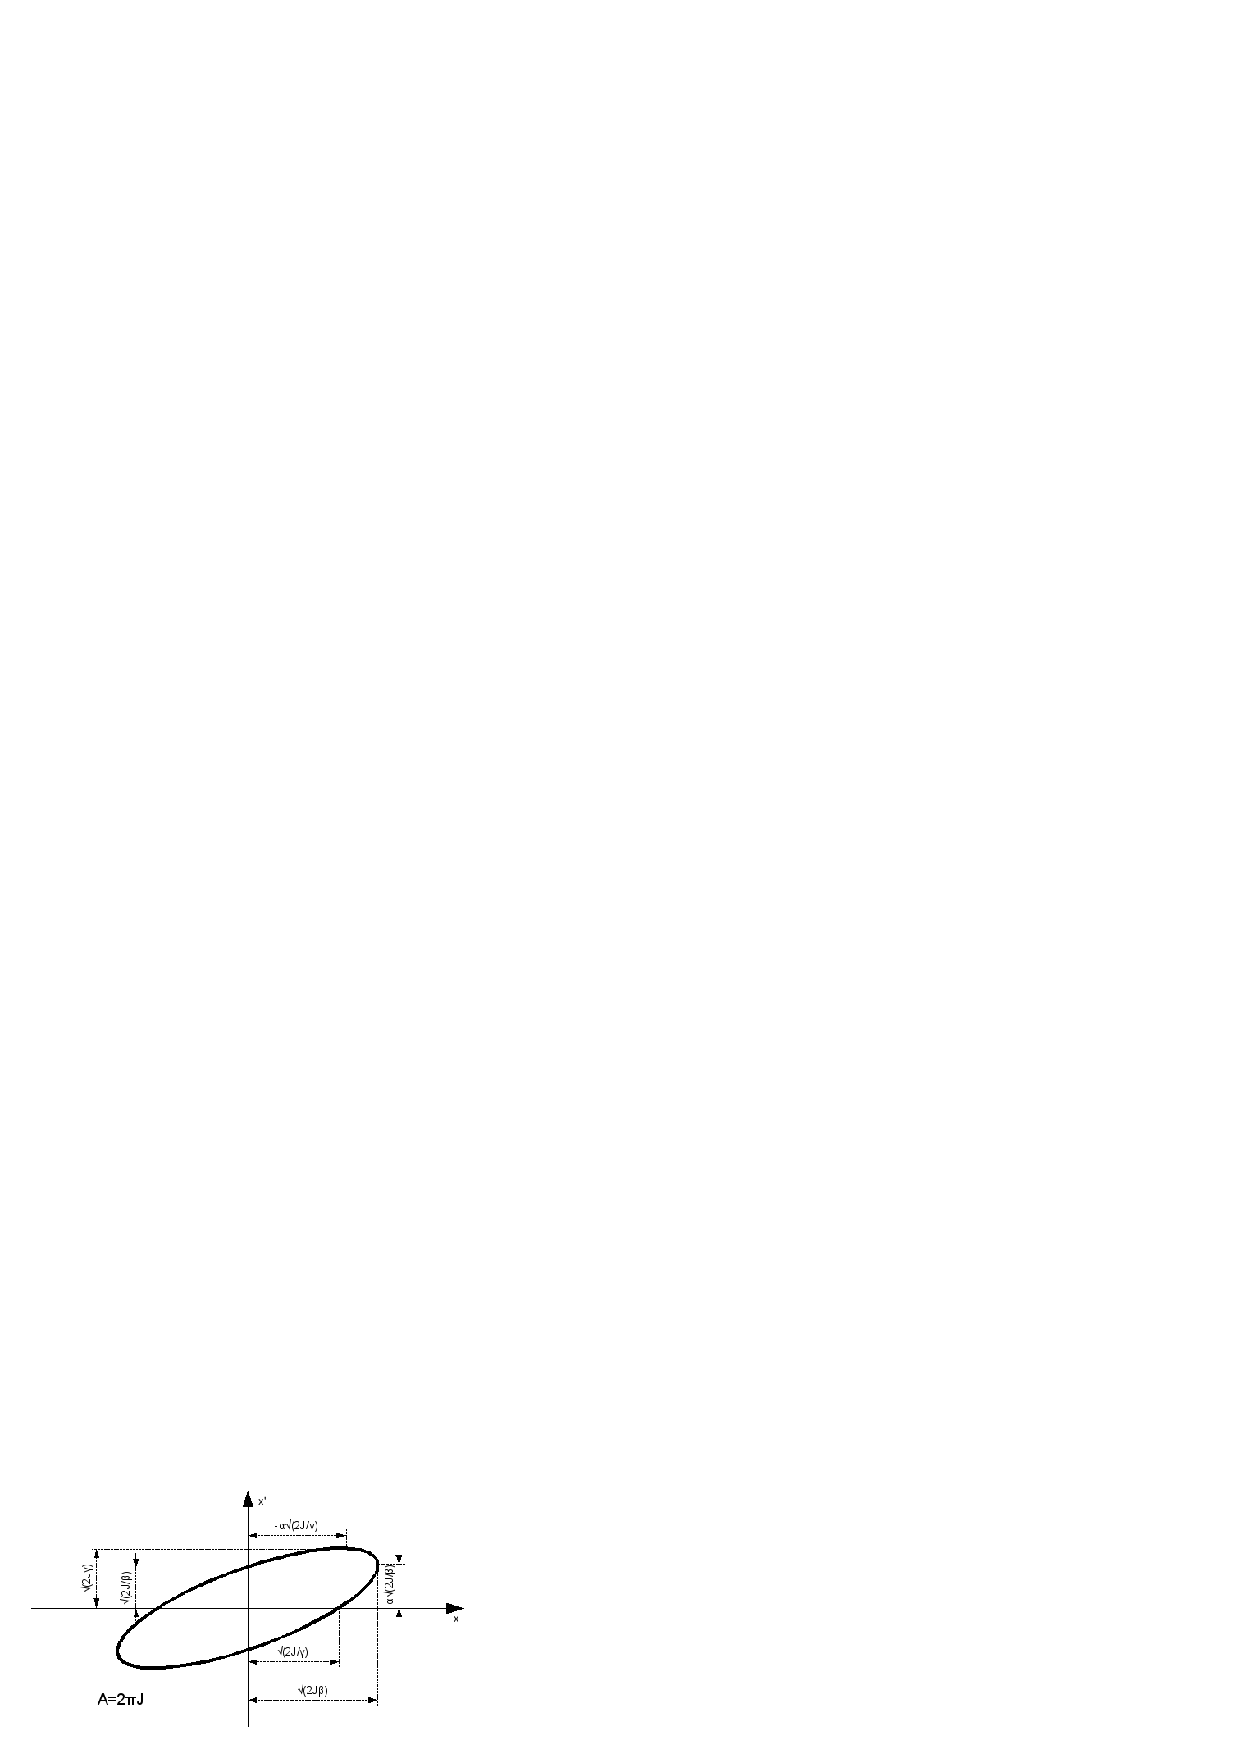
\includegraphics[scale=0.75]{phaseellipse.png}
	\caption{Anatomy of a phase space ellipse.  Modified from: H. Wiedemann, Particle Accelerator Physics I, 2nd ed., p.152.}
	\label{fig:ellipse}
\end{figure}

\section{The Gaussian distribution}
For a distribution of particles in phase space with density $\rho(J,\phi)$, we define the emittance to be
\Begineq
	\varepsilon = \langle J \rangle = \int dJ \, d\phi \, J\rho(J,\phi).
\Endeq
In these $(J,\phi)$ coordinates, a Gaussian phase space distribution can be represented as
\Begineq
	\rho(J,\phi) = \frac{1}{2\pi\varepsilon} e^{-\frac{J}{\varepsilon}}.
	\label{eq:rho}
\Endeq

This distribution is normalized to 1, i.e. $\int dJ \, d\phi \rho(J,\phi) = 1$.  Its emittance is $\varepsilon$, since
\Begineq
	\langle J \rangle = \int_{0}^{\infty} dJ \int_{0}^{2\pi} d\phi \, J \rho(J,\phi) = \frac{1}{\varepsilon} \int_{0}^{\infty} dJ \, J e^{-\frac{J}{\varepsilon}} = \varepsilon.
\Endeq
The rms beam size and divergence are
\begin{align}
	\sigma_x & = \sqrt{\langle x^2 \rangle} = \sqrt{\langle 2J\beta \cos^2 \phi \rangle} = \sqrt{\varepsilon\beta}  \\
	\sigma_{x'} & = \sqrt{\langle x'^2 \rangle} = \sqrt{\biggl\langle \frac{2J}{\beta} (\alpha \cos\phi + \sin\phi)^2 \biggr\rangle} = \sqrt{\varepsilon\gamma},
	\label{eq:rms}
\end{align}
while the covariance is
\Begineq
	\langle xx' \rangle = \langle -2J (\alpha \cos^2 \phi + \sin\phi \cos\phi) \rangle = -\varepsilon\alpha.
	\label{eq:corr}
\Endeq

\subsection{Alternate representation of the distribution}
Equations (\ref{eq:rms}) and (\ref{eq:corr}) lead to an alternative representation of the distribution, which replaces the Twiss parameters with rms quantities.
From the definition of $\gamma$, 
\Begineq
	\langle x'^2 \rangle = \varepsilon\frac{1+\alpha^2}{\beta} = \frac{\varepsilon^2 + \langle xx' \rangle^2}{\langle x^2 \rangle} \quad \Rightarrow \quad \varepsilon = \sqrt{\langle x^2 \rangle\langle x'^2 \rangle - \langle xx' \rangle^2}.
\Endeq
So, the distribution can be written
\Begineq
	\rho(x,x') = \frac{1}{2\pi\sqrt{\langle x^2 \rangle\langle x'^2 \rangle - \langle xx' \rangle^2}} \exp \left( -\frac{\langle x'^2 \rangle x^2 - 2 \langle xx' \rangle xx' + \langle x^2 \rangle x'^2}{2(\langle x^2 \rangle\langle x'^2 \rangle - \langle xx' \rangle^2)} \right)
\Endeq

\subsection{Implementation}
\begin{figure}[htp]
	\centering 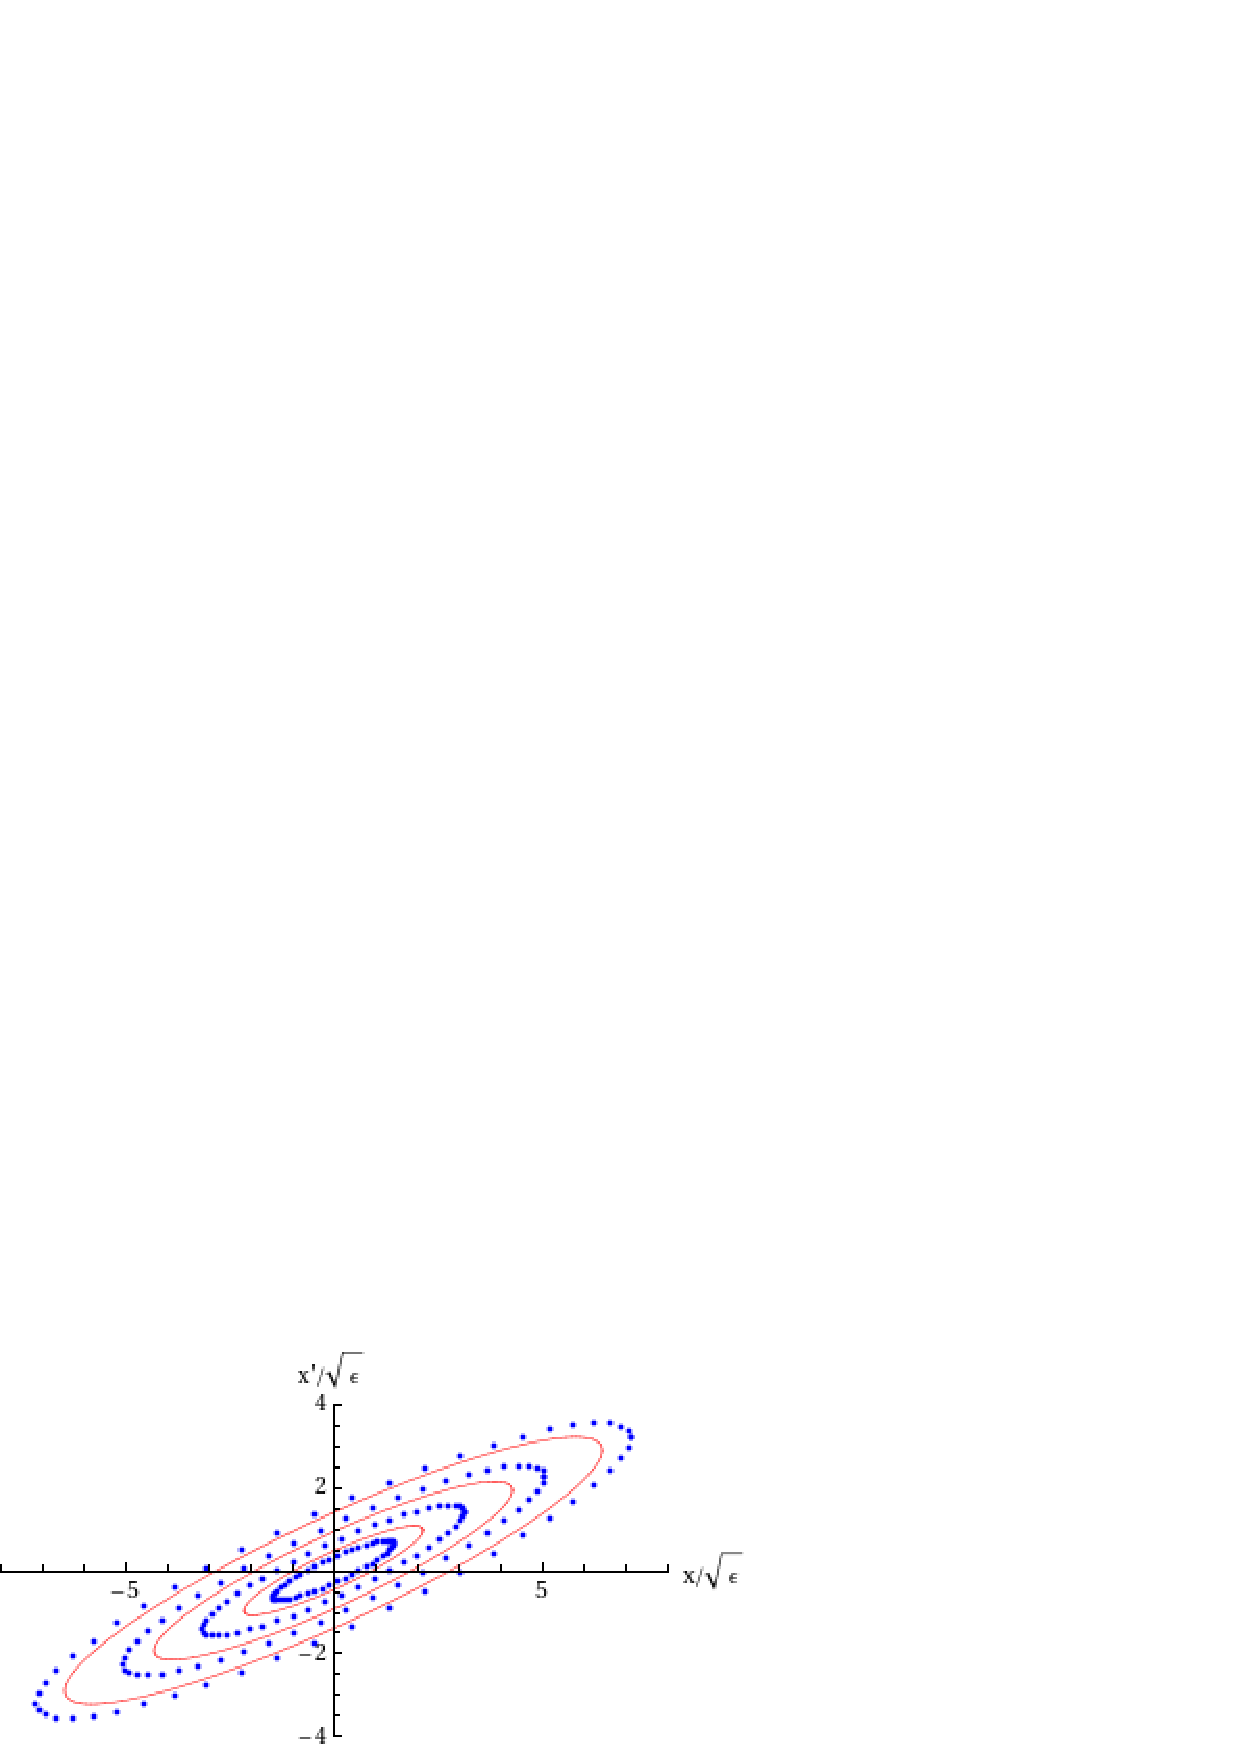
\includegraphics[scale=0.75]{filledellipse.png}
	\caption{We partition the phase space into regions bounded by ellipses (solid ellipses in red), and then calculate where to place the particles (dots in blue).  The red ellipses are placed so that their $\sqrt{J}$ increases by regular steps.  A number of blue ellipses of particles cover the region inside a certain cutoff radius, and one blue ellipse covers the region outside the largest red ellipse.  For this example, we set the cutoff at 3$\sigma$, have 3 ellipses in the inner region, and have 50 particles per ellipse.}
	\label{fig:finishedellipse}
\end{figure}

\begin{itemize}
\item Since we cannot represent the distribution with an infinite number of ellipses, we must implement some sort of sigma cutoff $g$ at which we will stop representing the distribution regularly --- commonly, $g$ is set to $3$ or $4$.  The space inside this sigma cutoff will be represented by a set of $N$ concentric ellipses; the space outside will be represented by a single ellipse.
\item Partition the inner region into $N$ sections $\lbrace S_{n} \rbrace, 1 \leq n \leq N$, each bounded by concentric boundary ellipses at $J = B_{n-1}$ and $B_{n}$, which will be calculated below.  $\sqrt{J}$ is increased by a constant amount from one boundary to the next, i.e. $\sqrt{B_{n}} = n\Delta$, $n = 0,...,N$.  Including the exterior section $S_{out}$, there are $N+1$ sections.
\item In each section $S_{n}$, place an ellipse of $M$ macroparticles at $J = J_{n}$.  Also place an ellipse at $J = J_{out}$ in $S_{out}$.  The macroparticles will be placed uniformly in $0 \leq \phi < 2\pi$.
\end{itemize}

The goal is to replace the Gaussian distribution given in equation \ref{eq:rho} with 
\Begineq
	\rho_{model}(J,\phi) = \left[ \sum_{n=1}^{N} q_{n} \, \delta(J - J_{n}) + q_{out} \, \delta(J - J_{out}) \right] \, \sum_{m=1}^{M} \frac{1}{M} \, \delta(\phi - 2\pi \frac{m}{M})
\Endeq
where each ring has a total weight $q_{n}$.  

We determine $\lbrace q_{n} \rbrace$, $\lbrace J_{n} \rbrace$, $q_{out}$, and $J_{out}$ by requiring that these conditions be satisfied:
\begin{itemize}
\item $\rho_{model}$ is normalized to 1,
\item $\langle J \rangle_{model} = \varepsilon$ for the entire distribution,
\item $q_{n} = \iint_{S_{n}} dJ d\phi \, \rho$ and $\langle J \rangle_{n} = \iint_{S_{n}} dJ d\phi \, J \rho$ agree between the model and Gaussian distributions, for each section $S_{n}$
\end{itemize}
That is, each ring carries the same weight and $\langle J \rangle$ as the section it represents, and the distribution as a whole has the same normalization and emittance.  In our partitioning, we are effectively doing the following:
\begin{align}
	1 & = \int_{0}^{\infty} dJ \int_{0}^{2\pi} d\phi \, \rho(J,\phi)                                                                                         \\
	  & = \sum_{n=1}^{N} \underbrace{\int_{B_{n-1}}^{B_{n}} dJ \int_{0}^{2\pi} d\phi \, \rho(J,\phi)}_{q_{n}} + \underbrace{\int_{B_{N}}^{\infty} dJ \int_{0}^{2\pi} d\phi \, \rho(J,\phi)}_{q_{out}}                                                                                                          \\
	\langle J \rangle & = \int_{0}^{\infty} dJ \int_{0}^{2\pi} d\phi \, J \, \rho(J,\phi)                                                                    \\
	                  & = \sum_{n=1}^{N} \underbrace{\int_{B_{n-1}}^{B_{n}} dJ \int_{0}^{2\pi} d\phi \, J \, \rho(J,\phi)}_{\langle J \rangle_{n}} + \underbrace{\int_{B_{N}}^{\infty} dJ \int_{0}^{2\pi} d\phi \, J \, \rho(J,\phi)}_{\langle J \rangle_{out}}.
\end{align}


The boundary ellipses lie at $J \in \lbrace B_{n} \rbrace, 0 \leq n \leq N$, where $B_{0} = 0$ characterizes the origin of the phase space coordinates.  If our sigma cutoff is $g$, the outermost boundary is defined by $\sqrt{B_{N}} = g \sqrt{\frac{\varepsilon}{2}}$, so
\Begineq
	B_{n} = g^2 \frac{n^2}{N^2} \frac{\varepsilon}{2}.
\Endeq

The requirement that, for each section, $q_n$ is the same for the model and the Gaussian distribution leads to 
\Begineq\begin{split}
	q_{n} & = \int_{B_{n-1}}^{B_{n}} dJ \int_{0}^{2\pi} d\phi \, \rho(J,\phi) = \frac{1}{\varepsilon} \int_{B_{n-1}}^{B_{n}} dJ \, e^{-\frac{J}{\varepsilon}} = \exp \left( -\frac{B_{n-1}}{\varepsilon} \right) - \exp \left( -\frac{B_{n}}{\varepsilon} \right),  \\
	q_{out} & = \int_{B_{N}}^{\infty} dJ \int_{0}^{2\pi} d\phi \, \rho(J,\phi) = \exp \left( -\frac{B_{N}}{\varepsilon} \right).
\end{split}\Endeq

The same constraint on $\langle J \rangle_n$ leads to
\Begineq\begin{split}
	q_{n}J_{n} & = \int_{B_{n-1}}^{B_{n}} dJ \, J \, \frac{1}{\varepsilon} e^{-\frac{J}{\varepsilon}} = \varepsilon \int_{\frac{B_{n-1}}{\varepsilon}}^{\frac{B_{n}}{\varepsilon}} d\xi \, \xi \, e^{-\xi} = \varepsilon (\xi + 1) e^{-\xi} \biggr\vert_{\frac{B_{n}}{\varepsilon}}^{\frac{B_{n-1}}{\varepsilon}},                              \\
	q_{out}J_{out} & = \int_{B_{N}}^{\infty} dJ \, J \, \frac{1}{\varepsilon} e^{-\frac{J}{\varepsilon}} = \varepsilon (\xi + 1) e^{-\xi} \biggr\vert_{\xi = \frac{B_{n}}{\varepsilon}}.
\end{split}\Endeq

\section{Final Results}
Our model distribution is
\Begineq
	\rho_{model}(J,\phi) = \left[ \sum_{n=1}^{N} q_{n} \, \delta(J - J_{n}) + q_{out} \, \delta(J - J_{out}) \right] \, \sum_{m=1}^{M} \frac{1}{M} \, \delta(\phi - 2\pi \frac{m}{M}).
\Endeq

Also, let us use dimensionless quantities $b_{n} = \frac{B_{n}}{\varepsilon} = \frac{g^2 n^2}{2 N^2}$.  The weight of each macroparticle is
\Begineq
	q_{n}/M = \frac{1}{M}(e^{-b_{n-1}} - e^{-b_{n}}),
\Endeq
\Begineq
	q_{out}/M = \frac{1}{M} e^{-b_{N}}.
\Endeq
The rings lie at positions
\Begineq
	J_{n} = \varepsilon \, \frac{(b_{n-1}+1) e^{-b_{n-1}} - (b_{n}+1) e^{-b_{n}}}{e^{-b_{n-1}} - e^{-b_{n}}},
\Endeq
\Begineq
	J_{out} = \varepsilon (b_{N}+1).
\Endeq


\section{Ellipse representation of a Kapchinsky-Vladimirsky distribution}

\textit{Written by Michael Saelim}

In a four-dimensional phase space $(x,x',y,y')$, the Kapchinsky-Vladimirsky distribution presents a constant density in a three-dimensional subspace.  A four-dimensional Gaussian distribution can be written as an integral over K-V distributions..  We represent this phase space by a series of concentric ellipses on which macroparticles of equal weight are placed.  This adds more macroparticles to the exterior of the distribution, which aids observing nonlinear effects on the beam's transverse phase planes.

\subsection{Transformation to $(I,\phi)$ coordinates}
The canonical transformation between $(J,\phi)$ and $(x,x')$ coordinates has already been computed.  Now consider a 4D phase space $(x,x',y,y')$.  Using this framework, a 4D Gaussian distribution is
\begin{align}
	\rho(J_x,\phi_x,J_y,\phi_y) & = \frac{1}{(2\pi)^2 \varepsilon_x \varepsilon_y}\; exp(-\frac{J_x}{\varepsilon_x})\; exp(-\frac{J_y}{\varepsilon_y}) \\
	                            & = \frac{1}{(2\pi)^2 \varepsilon_x \varepsilon_y}\; exp(-\frac{I_1}{\varepsilon}),
\end{align}
where we have used a new set of orthogonal action coordinates:
\begin{align}
	I_1 & = \left( \frac{J_x}{\varepsilon_x} + \frac{J_y}{\varepsilon_y} \right) \varepsilon  \\
	I_2 & = \left( -\frac{J_x}{\varepsilon_y} + \frac{J_y}{\varepsilon_x} \right) \varepsilon
\end{align}
with $\varepsilon = (\frac{1}{\varepsilon_x^2} + \frac{1}{\varepsilon_y^2})^{-1/2}$.  The reverse transformation is also noted:
\begin{align}
	J_x & = \left( \frac{I_1}{\varepsilon_x} - \frac{I_2}{\varepsilon_y} \right) \varepsilon  \\
	J_y & = \left( \frac{I_1}{\varepsilon_y} + \frac{I_2}{\varepsilon_x} \right) \varepsilon.
\end{align}

The K-V distribution is
\Begineq
	\rho(I_1,I_2,\phi_x,\phi_y) = \frac{1}{A} \delta(I_1 - \xi),
\Endeq
where $A = \frac{\varepsilon_x \varepsilon_y}{\varepsilon^2} \xi (2\pi)^2$ is a constant which normalizes the distribution to 1.  By choosing a particular $\xi$ and iterating over the domain of the three remaining coordinates, one can populate a 3D subspace of constant density.

The range in $I_2$ to be iterated over is constrained by $J_x$, $J_y \geq 0$.  $J_x, J_y = 0$ give the limits $I_2 \in [-\frac{\varepsilon_x}{\varepsilon_y} I_1, \frac{\varepsilon_y}{\varepsilon_x} I_1]$.  This range is divided into N regions of equal size, with a ring of macroparticles placed in the middle of each region.  The angle variables are also constrained to $\phi_x, \phi_y \in [0, 2\pi]$, with each range divided into $M_x$ and $M_y$ regions, respectively.  Each of these regions will have a particle placed in its center.

The weight of a macroparticle is determined by the total weight of the region of phase space it represents.  Because the density $\rho$ is only dependent on $I_1$,
\begin{align}
	q & = \int_{0}^{\infty} dI_1 \int_{I_2}^{I_2 + \Delta I_2} dI_2 \int_{\phi_x}^{\phi_x + \Delta \phi_x} d\phi_x \int_{\phi_y}^{\phi_y + \Delta \phi_y} d\phi_y \; \frac{1}{A} \delta(I_1 - \xi) \\
	  & = \frac{1}{A} \Delta I_2 \Delta \phi_x \Delta \phi_y.
\end{align}
To represent the distribution with macroparticles of equal weight, we must partition $(I_2,\phi_x,\phi_y)$-space into regions of equal volume.

The weight of each macroparticle is
\Begineq
	q = \frac{1}{N M_x M_y} = \frac{1}{number of particles}
\Endeq


\subsection{Sidenote: Canonical nature of the transformation}
It can be shown that the transformation between $(J,\phi)$ and $(x,x')$ is canonical because the Jacobian matrix $\mathbf{M} = \frac{\partial(x,x')}{\partial(J,\phi)}$ is symplectic ($\mathbf{M}\mathbf{J}\mathbf{M}^T = \mathbf{J}$ for $\mathbf{J} = (\begin{smallmatrix} 0 && 1 \\ -1 && 0 \end{smallmatrix})$).

While the transformation between $(I_1,I_2,\phi_x,\phi_y)$ and $(J_x,J_y,\phi_x,\phi_y)$ is not canonical, its Jacobian determinant $\left\vert\frac{\partial(I_1,I_2,\phi_x,\phi_y)}{\partial(J_x,J_y,\phi_x,\phi_y)}\right\vert$ is still 1.

To create a canonical transformation, new angle coordinates must also be defined in the same manner as the new action coordinates:
\begin{align}
	\psi_1 & = \left( \frac{\phi_x}{\varepsilon_x} + \frac{\phi_y}{\varepsilon_y} \right) \varepsilon  \\
	\psi_2 & = \left( -\frac{\phi_x}{\varepsilon_y} + \frac{\phi_y}{\varepsilon_x} \right) \varepsilon
\end{align}

Transforming both action and angle coordinates is canonical, because $\mathbf{M}\mathbf{J}\mathbf{M}^T = \mathbf{J}$ for the Jacobian matrix $\mathbf{M} = \frac{\partial(I_1,I_2,\psi_1,\psi_2)}{\partial(J_x,J_y,\phi_x,\phi_y)}$ and $\mathbf{J} = (\begin{smallmatrix} 0 && \mathbf{I} \\ -\mathbf{I} && 0 \end{smallmatrix})$ where $\mathbf{I}$ is the 2x2 identity matrix.

While the limits of iteration for $I_2$ stays the same, the limits for $\psi_1$ and $\psi_2$ are more complicated, since they are constrained by $\phi_1,\phi_2 \in [0,2\pi]$.  The $\lbrace\phi\rbrace \rightarrow \lbrace\psi\rbrace$ transformation rotates the axes, so that the range to iterate over in $\psi_2$ is dependent on the value of $\psi_1$, which is not fixed, and vice versa.  
\begin{figure}[htp]
	\centering
	\begin{tabular}{c c}
	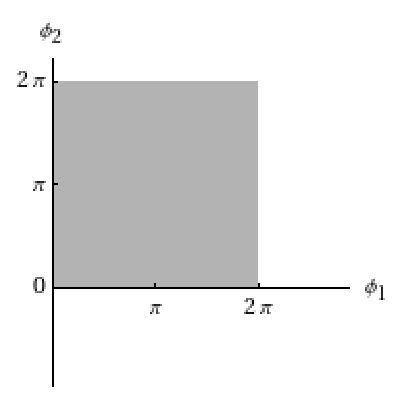
\includegraphics[scale=0.6]{phiblock.eps} & 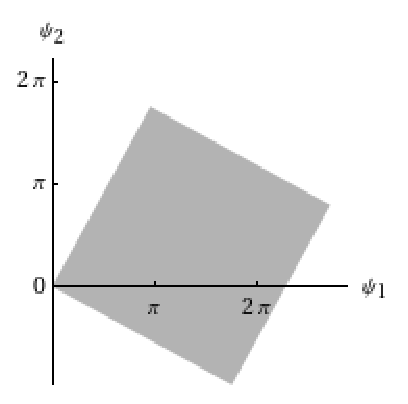
\includegraphics[scale=0.6]{psiblock.eps} \\
	(a) & (b)
	\end{tabular}
	\caption{The region to iterate over in $\lbrace\phi\rbrace$-space (a) is subject to a rotation of axes to $\lbrace\psi\rbrace$-space (b).}
	\label{fig:phipsi}
\end{figure}

However, iterating over this region need not occur along the $\psi_1,\psi_2$ axes, as long as a constant density of points is maintained.  So instead of iterating horizontally over $\psi_1$ and vertically over $\psi_2$, it is possible to iterate diagonally along the axes formed by the edges of the square - but, this is the same as iterating over $\phi_1$ and $\phi_2$, because $\left\vert\frac{\partial(\psi_1,\psi_2)}{\partial(\phi_x,\phi_y)}\right\vert = 1$.

Therefore, the weight of each macroparticle is as before:
\Begineq
	q = \frac{1}{A} \Delta I_2 \Delta \phi_x \Delta \phi_y.
\Endeq
\chapter{Creating a regular initial beam distribution in \bmad}

\section*{Introduction}
This addition to \bmad allows the initialization of beam distributions where the points are not selected randomly in phase space.  Three distributions are available: 
\begin{itemize}
\item \vn{grid} places a non-Gaussian, rectangular grid of points on a 2D phase plane.  This can also be uesd to create a line of points or a single point.  
\item \vn{ellipse} represents a 2D Gaussian distribution by concentric ellipses of macroparticles.
\item \vn{KV} represents a 4D Kapchinsky-Vladimirsky distribution, which presents a constant density at all points.  This phase space is also represented by a series of concentric ellipses of macroparticles.  
\end{itemize}
\vn{ellipse} and \vn{KV} especially help visualize nonlinear effects on the beam's transverse phase planes, as they are most visible on the tails of the distribution, which are usually underrepresented in a distribution where points are selected randomly.

\section*{General settings}
As with random distributions, the beam is initialized with the \vn{init_beam_distribution} subroutine, but now \vn{%beam_init_struct} contains two new members: \vn{%is_random} and \vn{%regular_beam_init}.

The trigger \vn{%is_random} determines whether \vn{init_beam_distribution} randomly generates points in a Gaussian distribution or generates regular distributions.  It is set to \vn{.true.} by default.

\vn{%regular_beam_init} is itself a struct containing all the pertinent information for constructing a regular beam distribution, with members that hold information for every type of distribution.  Many of these members are arrays, whose three components correspond to the phase planes $(x,p_x)$, $(y,p_y)$, and $(z,p_z)$.  All members of the struct are initialized to zero.  Also, \vn{%n_particle} is now automatically calculated from parameters contained in \vn{%regular_beam_init}.  

The following sections enumerate the different distributions available and explain their settings in \vn{%regular_beam_init}.

\section*{The grid distribution}
The \vn{grid} distribution is triggered by setting \vn{regular_beam_init%type} to \vn{grid\$}.  \vn{%n_x} and \vn{%n_px} set the number of columns and rows, respectively, and \vn{%minima} and \vn{%maxima} set the lower and upper limits in the directions $(x,p_x,y,p_y,z,p_z)$.  This distribution can also be used to specify a single point in the plane by setting both \vn{%n_x} and \vn{%n_px} to 1.

\section*{The ellipse distribution}
For a 2D Gaussian distribution, the contours of constant density form concentric ellipses.  The \vn{ellipse} distribution represents this using concentric ellipses of uniformly-spaced macroparticles.  A region out to \vn{%sigma_cutoff} standard deviations is represented by \vn{%n_interior} ellipses, and the region outside this cutoff is represented a single ellipse.  Each ellipse is then uniformly populated with \vn{%part_per_ellipse} appropriately-weighted macroparticles.  Twiss parameters, emittances, and other parameters for the beam are derived from the \vn{ele_struct} and \vn{beam_init_struct}.

For more information, see the theoretical discussion on this distribution.

\section*{The K-V distribution}
The 4D Kapchinsky-Vladimirsky distribution exhibits a constant density profile, represented using concentric ellipses of uniformly-spaced macroparticles with equal weight.  Using the K-V distribution requires that two phase planes be marked with \vn{%type} $=$ \vn{KV\$}.  The program iterates over \vn{%n_I2} equally-spaced steps in the I2-direction, populating each ring with \vn{%part_per_ellipse} equally-weighted macroparticles.  \vn{%A} $= \frac{I_1}{\varepsilon}$ must also be set.  Explanations of what these quantities are can be found in the theoretical discussion of the K-V distribution.  Twiss parameters, emittances, and other parameters for the beam are derived from the \vn{ele_struct} and \vn{beam_init_struct}.

For more information, see the theoretical discussion on this distribution.


\end{document}